% TODO: The bibfile is very wrong in citing everything (webpages, chapters of a page, etc) as @article -- fix it

\documentclass[a4paper]{amsart}

\usepackage{textcomp}
\usepackage{amsmath}
\usepackage{amsthm}
\usepackage{amsfonts}
\usepackage{amssymb}
\usepackage{hyperref}
\usepackage{cleveref}
\usepackage{comment}
\usepackage{enumitem}
\usepackage{svg}
\usepackage{float}
\usepackage{xcolor}
\usepackage{tkz-base}
\usepackage{subfig}

\usepackage[backend=bibtex]{biblatex}
\addbibresource{main.bib}

\theoremstyle{plain}
\newtheorem{theorem}{Theorem}
\newtheorem{lemma}{Lemma}
\newtheorem{corollary}{Corollary}
\newtheorem{remark}{Remark}
\newtheorem{conjecture}{Conjecture}
\theoremstyle{definition}
\newtheorem{definition}{Definition}

\floatplacement{figure}{h}

\begin{document}

\title[\(n^2 + 1\) unit vertical triangles cannot cover a triangle of side \(> n\)]{\(n^2 + 1\) unit equilateral triangles cannot cover an equilateral triangle of side \(> n\) if all triangles have parallel sides}

\author{Jineon Baek}
\address{University of Michigan - Ann Arbor}
\email{jineon@umich.edu}
\author{Seewoo Lee}
\address{University of California - Berkeley}
\email{seewoo5@berkeley.edu}

\begin{abstract}
Conway and Soifer showed that an equilateral triangle \(T\) of side \(n + \varepsilon\) with sufficiently small $\varepsilon > 0$ can be covered by \(n^2 + 2\) unit equilateral triangles.
They conjectured that it is impossible to cover $T$ with \(n^2 + 1\) unit equilateral triangles no matter how small $\varepsilon$ is.

We show that if we require the sides of all triangles to be parallel to the sides of \(T\) (e.g. $\bigtriangleup$ and $\bigtriangledown$), then it is impossible to cover \(T\) with \(n^2 + 1\) unit equilateral triangles for any $\varepsilon > 0$.
As the coverings of $T$ by Conway and Soifer only involve triangles with parallel sides,
our result determines the exact minimum number $n^2+2$ of unit equilateral triangles with parallel sides required to cover $T$.

Using our method, we also determine the largest value $\varepsilon = 1/n$ such that the vertical triangle $T$ of side $n + \varepsilon$ can be covered by $n^2+2$ vertical equilateral triangles,
which is achieved by the construction of Conway and Soifer.
\end{abstract}

\maketitle

\section{Introduction}

Conway and Soifer provided two ways to cover an equilateral triangle $T$ of side $> n$ with \(n^2 + 2\) unit equilateral triangles, and conjectured that $n^2 + 1$ unit equilateral triangles cannot cover $T$ \cite{conway2004coverup, conway2005covering}.
Their paper was famously short, and was deliberately made so by the authors as an attempt to set the world record for the shortest math paper ever; see \cite{soifer2009coffee} for the full story by the second author.

\begin{figure}[h]
\centering
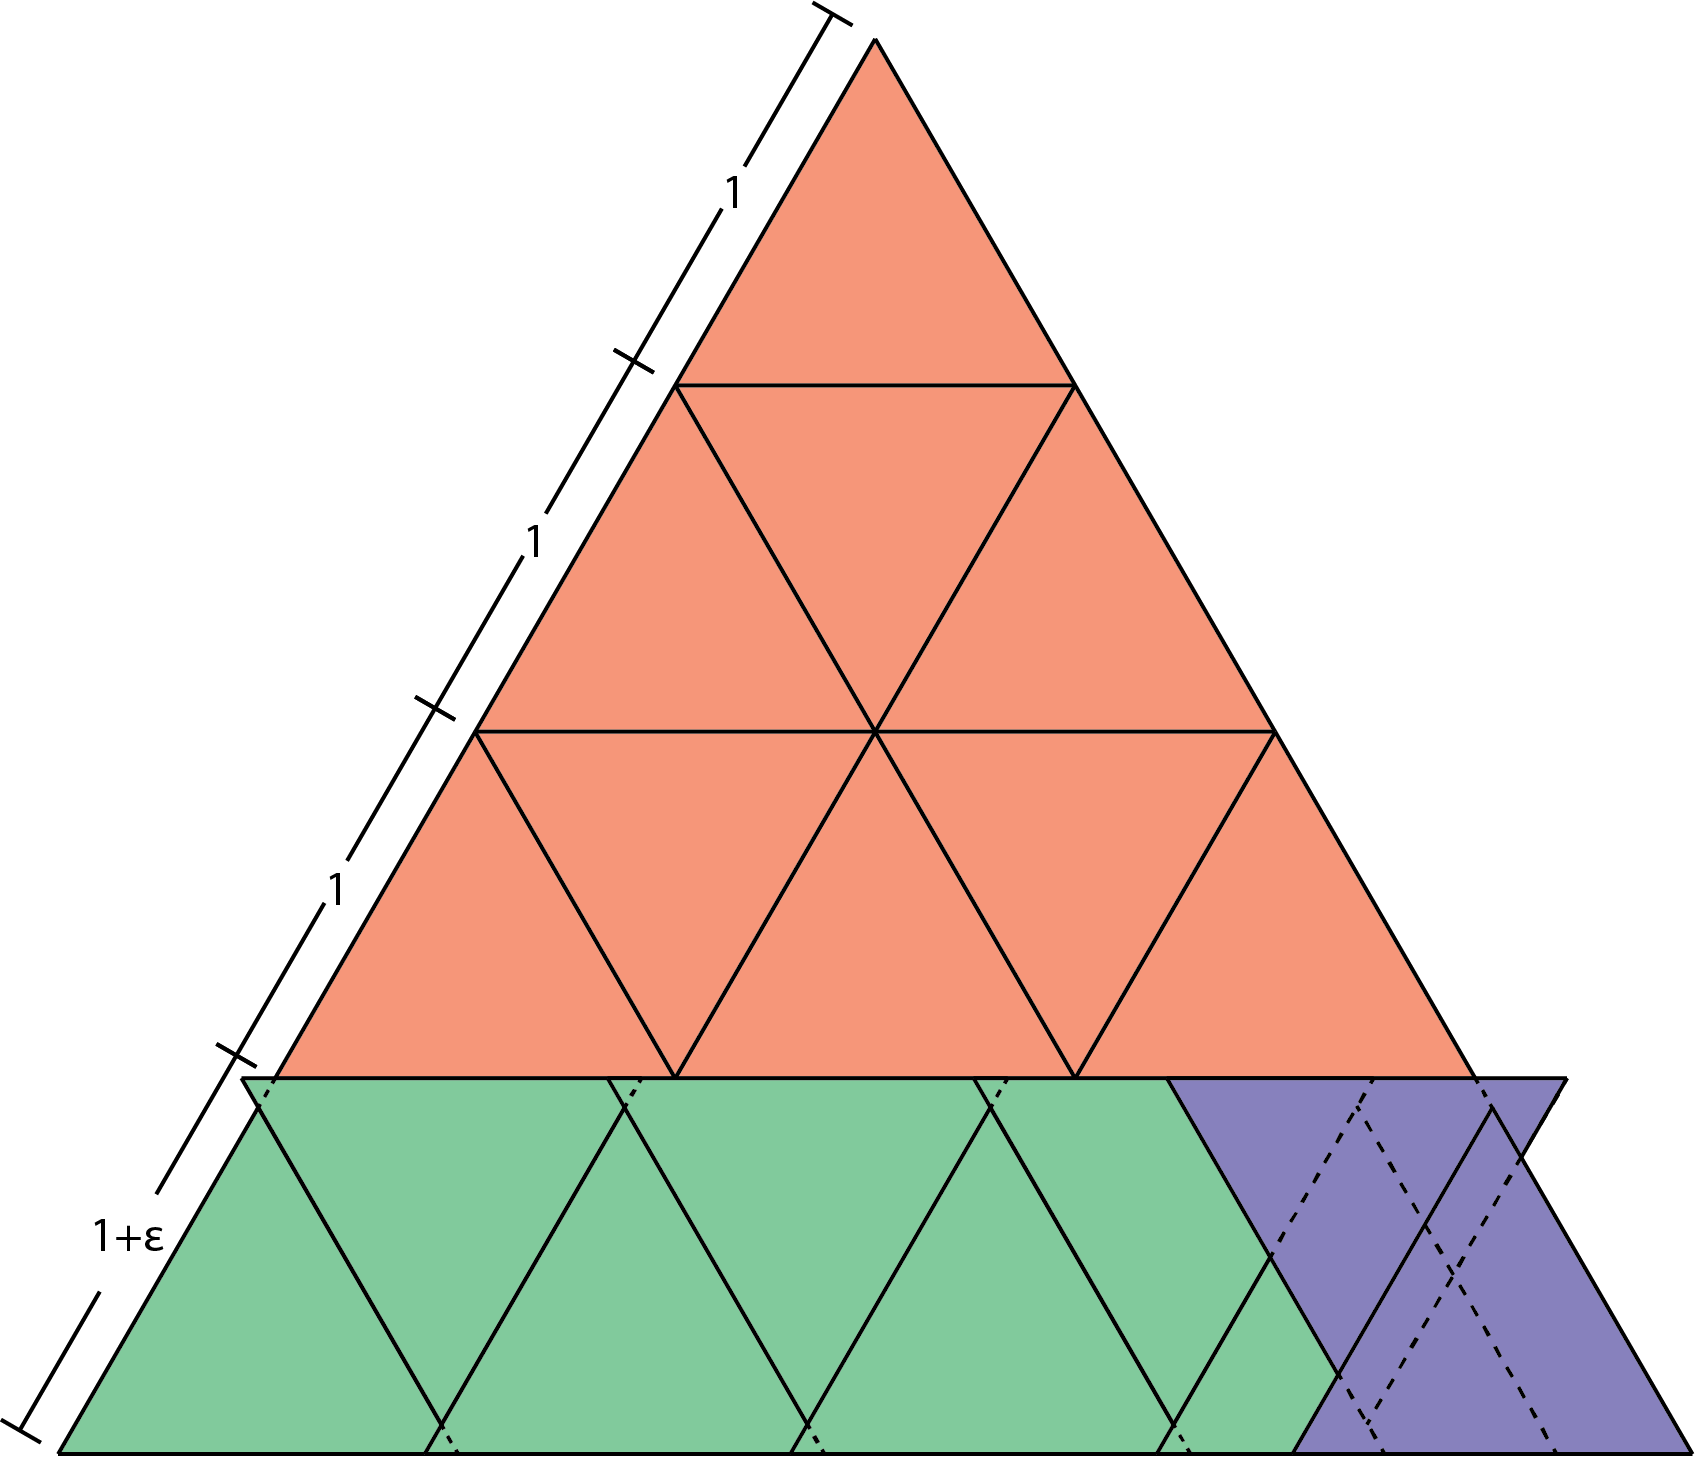
\includegraphics[width=0.5\linewidth]{triangle1.png}
\caption{}
\label{fig:triangle1}
\end{figure}

\begin{comment}
\begin{figure}[h]
   \begin{minipage}{0.5\textwidth}
     \centering
     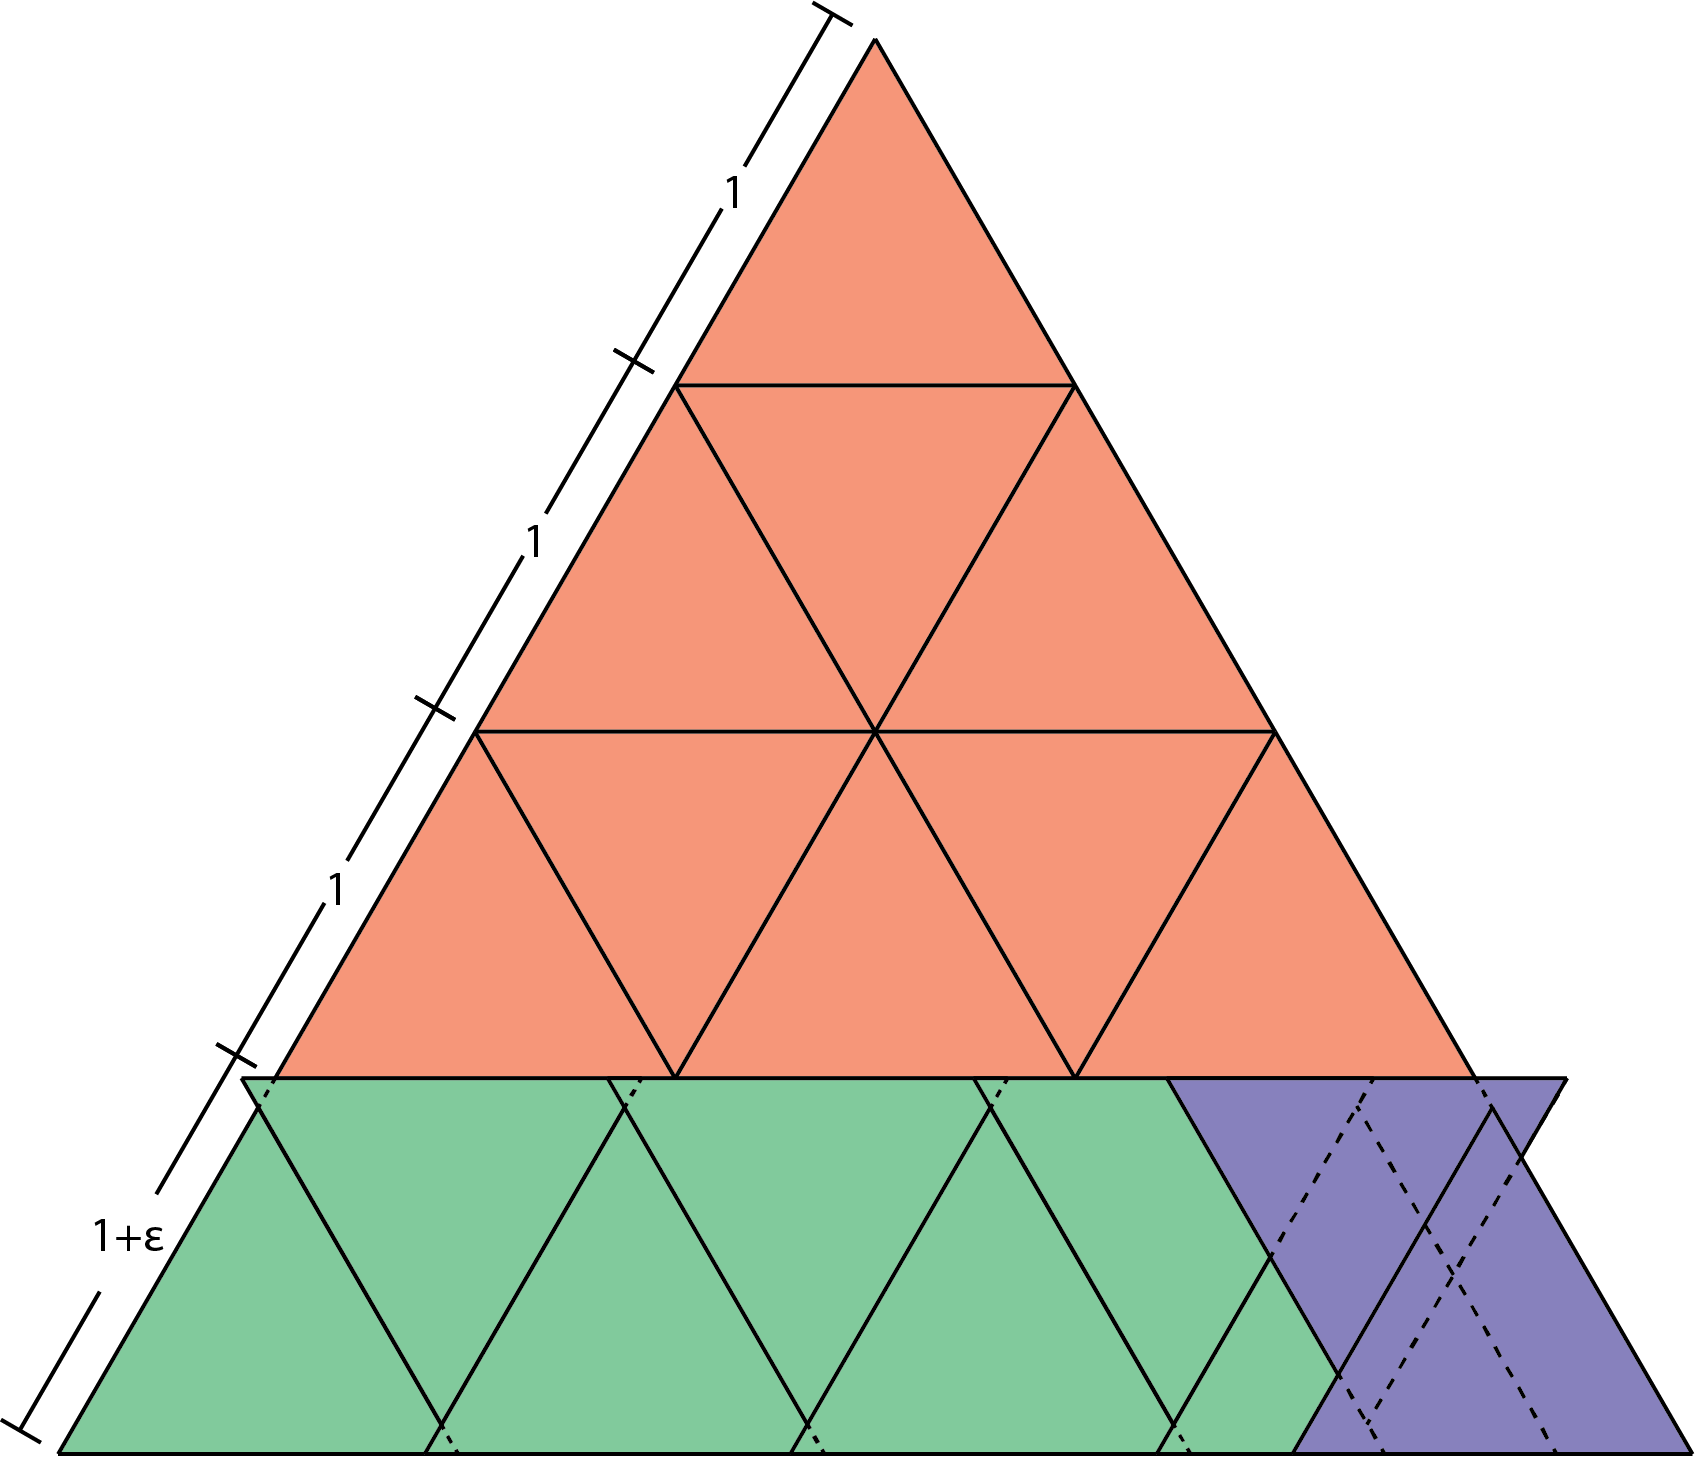
\includegraphics[width=0.9\linewidth]{triangle1.png}
     \caption{}
     \label{fig:triangle1}
   \end{minipage}\hfill
   \begin{minipage}{0.5\textwidth}
     \centering
     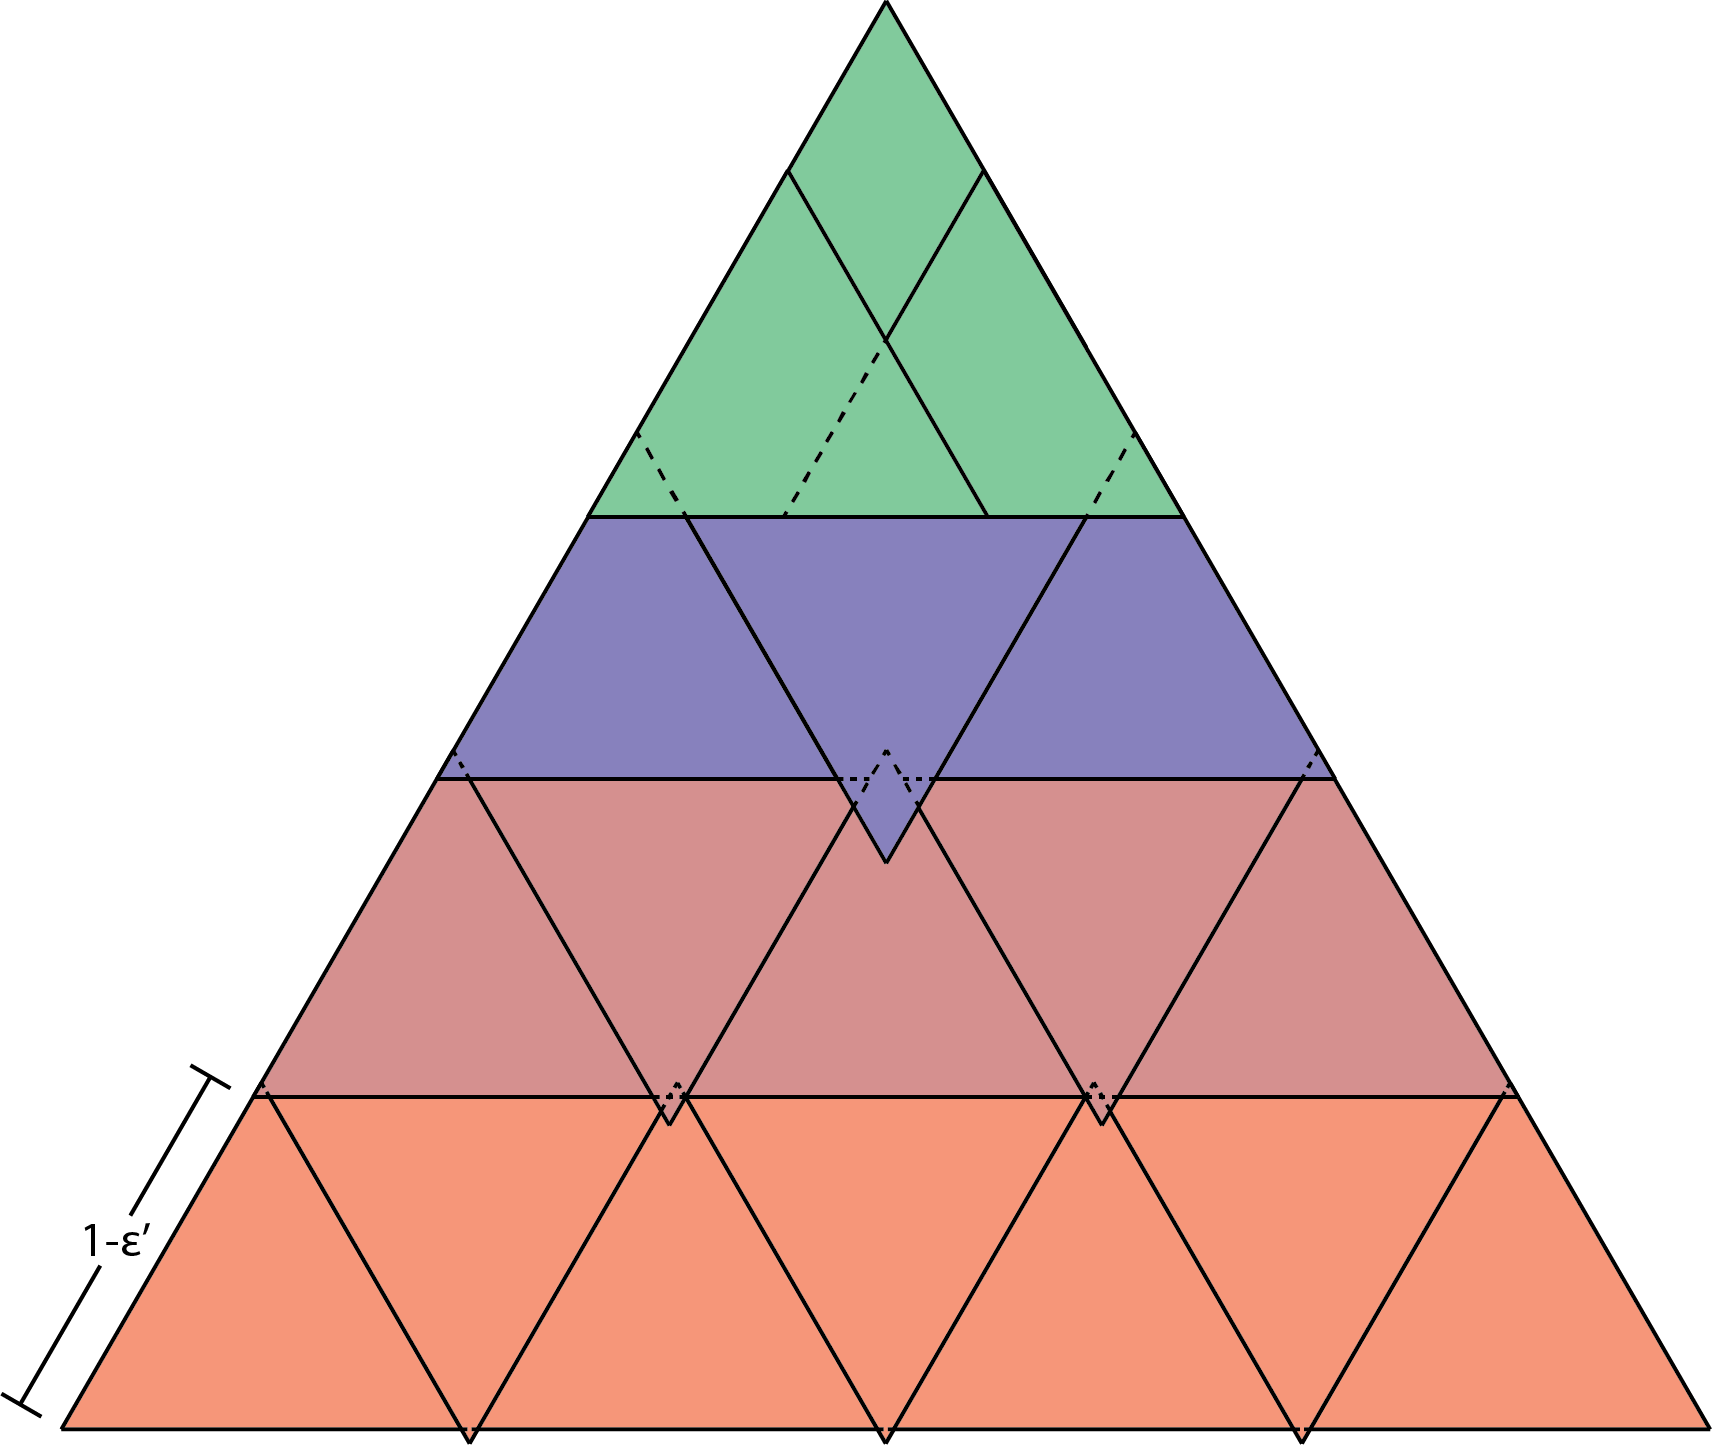
\includegraphics[width=0.9\linewidth]{triangle2.png}
     \caption{}
     \label{fig:triangle2}
   \end{minipage}
\end{figure}

For Figure \ref{fig:triangle1}, we first cover the upper part of the original equilateral triangle of side length $n+\epsilon$ equilateral triangle of side length $n-1$ with $(n-1)^2$ triangles (light red triangles). After that, the remaning part is a trapezoid of lengths $1+\epsilon$, $n+\epsilon$, $1+\epsilon$, and $n-1$. Now put $2n-2$ triangles from left, alternatively (green triangles), then we can check that the remaining part is a parallelogram of lengths $1+\epsilon$ and $\epsilon n$, minus a small equilateral triangle of length $\epsilon$ on the left-upper corner.
This can be covered with 2 triangles if $\epsilon \leq 1 / (n + 1)$ (blue triangles).
\newline
For Figure \ref{fig:triangle2}, we cover the large triangle from the bottom. We first cover the bottom layer with $n$ upward triangles and $n-1$ downward triangles, with $\epsilon' = \epsilon / (n-1)$ deviations (light red triangles). Then the resulting shape is a trapezoid of lengths $1 - \epsilon'$, $n +(n-1)\epsilon'$, $1 - \epsilon'$, and $n - 1 + n\epsilon'$, with small ``bump" triangles of lengths $\epsilon'$. Now we stack the next bottom layer with $n-1$ upward triangles and $n-2$ downward triangles, with $\epsilon''$ deviations. To cover the upper side of the light red trapezoid tightly, our new $\epsilon''$ should satisfy $(n-1) + (n-2)\epsilon'' = (n-1) + n\epsilon'$, hence $\epsilon'' = n\epsilon' / (n-2)$. Continue this until you stack up the total $(n-1)$ layers, where the top layer (blue triangles) consists of 2 upward triangles and 1 downward triangle with deviation
$$
\frac{n}{n-2} \frac{n-1}{n-3} \frac{n-2}{n-4} \cdots \frac{3}{1} \epsilon' = \frac{n(n-1)}{2} \epsilon' = \frac{n}{2} \epsilon.
$$
The remaining part of the triangle can be covered with three triangles of unit lengths if $1 + 2\cdot \frac{n}{2}\epsilon \le \frac{3}{2}$, i.e. if $\epsilon \leq \frac{1}{2n}$.
\end{comment}


\begin{theorem}[Conway and Soifer \cite{conway2004coverup, conway2005covering}]
\label{thm:main-prev}
$n^2 + 2$ unit equilateral triangles can cover an equilateral triangle $T$ of side $n + \varepsilon$ for a sufficiently small $\varepsilon > 0$.
\end{theorem}

\begin{conjecture}[Conway and Soifer \cite{conway2004coverup}]
\label{conj:main}
$n^2 + 1$ unit equilateral triangles cannot cover an equilateral triangle $T$ of side $n + \varepsilon$ for any $\varepsilon > 0$.
\end{conjecture}

\begin{comment}
In \Cref{fig:triangle1}, Conway used $(n-1)^2$ triangles to cover the upper part of $T$ with side $n-1$.
This leaves the trapezoid with  height slightly greater than 1 and the bottom side slightly larger than $n$ uncovered.
He then slightly misaligns the remaining $2n + 1$ triangles to cover the trapezoid.
In \Cref{fig:triangle2}, Soifer used $2n - 1$ triangles to cover a trapezoid of bottom side $n$ and height slight less than 1.
By stacking such $n-1$ trapezoids of height slightly less than 1 and decreasing width, we are left with a single triangle of side $> 1$, and he covers the remaining triangle with three unit triangles.
\end{comment}

Related, Karabash and Soifer showed that for every non-equilateral triangle \(T\), \(n^2 + 1\) triangles similar to \(T\) and with the ratio of linear sizes \(1: (n + \varepsilon)\) can cover \(T\) \cite{karabash2005covering},
so the ``equilaterality'' is essential for \Cref{conj:main} to be true \cite{conway2004coverup, soifer2009coffee}.
Also, Karabash and Soifer generalized the coverings of Conway and Soifer and showed that a \emph{trigon}\footnote{A connected shape formed by unit equilateral triangles with matching edges.} made of \(n\) unit equilateral triangles can be covered by \(n + 2\) triangles of side \(1 - \varepsilon\) \cite{karabash2005covering}.
A similar problem of covering a square of side \(n + \varepsilon\) with unit squares has been also extensively studied \cite{karabash2006sharp, karabash2008note, chung2009packing, wang2016new, chungEfficientPackingsUnit2020}.
Still, to the best of the authors' knowledge, the original \Cref{conj:main} raised by Conway and Soifer hasn't been addressed directly in the literature.

Define an equilateral triangle as \emph{vertical} if one side of the triangle is parallel to the $x$-axis.
Note that both triangles $\bigtriangleup$ and $\bigtriangledown$ are vertical, and all the unit triangles used in Conway and Soifer's constructions (\Cref{fig:triangle1} and \ref{fig:triangle2}) are vertical.
Also, the generalized covering of trigons by Karabash and Soifer \cite{karabash2005covering} only uses vertical triangles as well.
Thus, it is natural to ask if one can cover the equilateral triangle of side \(> n\) with \(n^2 + 1\) vertical unit triangles.
In this paper, we show that it is impossible.

\begin{theorem}

\(n^2 + 1\) unit vertical equilateral triangles cannot cover an vertical equilateral triangle of side \(> n\).

\label{thm:triangle-cover-cor}
\end{theorem}

Our proof generalizes to an arbitrary union \(X\) of \(n\) vertical triangles with disjoint interiors: it is impossible to cover \(X\) with \(n + 1\) vertical equilateral triangles of side \(< 1\).

\begin{theorem}

Let \(X\) be any union of \(n\) unit vertical equilateral triangles \(S_1, S_2, \dots, S_n\) with disjoint interiors. Then \(X\) cannot be covered by \(n + 1\) vertical equilateral triangles of sides less than one.

\label{thm:triangle-cover}
\end{theorem}

To recover \Cref{thm:triangle-cover-cor} from \Cref{thm:triangle-cover}, assume by contradiction that an vertical equilateral triangle \(T\) of side \(> n\) can be covered by \(n^2 + 1\) unit vertical equilateral triangles. Shrink the covering so that \(T\) have side exactly \(n\) and the small triangles have side \(< 1\). Then we get contradiction by \Cref{thm:triangle-cover} as \(T\) is a union of \(n^2\) unit vertical triangles with disjoint interiors.
As the coverings of \(T\) by Conway and Soifer (\Cref{fig:triangle1} and \ref{fig:triangle2}) and the coverings of trigons by Karabash and Soifer only uses vertical triangles,
we match the exact minimum number of unit vertical equilateral triangles required for covering.

\begin{corollary}
The minimum number of unit vertical equilateral triangles required to cover a vertical equilateral triangle of side \(n + \varepsilon\) with a sufficiently small $\varepsilon > 0$ is exactly \(n^2+2\).

Also, the minimum number of unit vertical triangles required to cover a trigon made of \(n\) vertical equilateral triangles of side \(1 + \varepsilon\) with a sufficiently small $\varepsilon > 0$ is exactly \(n + 2\).

\label{cor:triangle-cover-number}
\end{corollary}

It is then natural to ask for the maximum possible $\varepsilon > 0$ such that the equilateral triangle of side $n + \varepsilon$ can be covered by $n^2+2$ unit triangles.
For the equivalent problem on squares, it has been shown that (TODO).
If we require all triangles to be vertical, then our method can be used to determine the maximum value of $\varepsilon$.

\begin{theorem}
The largest value of $\varepsilon > 0$ such that the vertical triangle $T$ of side $n + \varepsilon$ can be covered by $n^2+2$ vertical equilateral triangles is $\varepsilon = 1/(n+1)$.
\label{thm:max-epsilon}
\end{theorem}

The maximum value is achieved by the first construction of \cite{conway2004coverup} (see \Cref{fig:triangle1}).
Note that for this $\varepsilon$, the area of the triangle of side $n + \varepsilon$ is $(n + 1/(n+1))^2 = n^2 + 2n/(n+1) + 1/(n+1)^2$ times the area of a unit equilateral triangle,
so the best covering has an area loss by $2/(n+1) - 1/(n+1)^2$. 

\section{Proof of \Cref{thm:triangle-cover}}

Take the standard Cartesian \(xy\)-coordinate system of a plane.
Inside the plane, take the triangular grid of unit equilateral triangles with the \(x\)-axis as one of the three axes of the triangular grid.

\begin{definition}
For every vertical triangle \(T\), define its rescaled \(y\)-coordinate \(z_T\) as the \(y\)-coordinate of the horizontal side of $T$ divided by \(\sqrt{3}/2\).
\label{def:rescaled-coord}
\end{definition}

Note that \(\sqrt{3}/2\) is the height of a unit equilateral triangle, so the value of \(z_T\) is an integer for every unit triangle \(T\) in the triangular grid.

\begin{definition}
For every vertical triangle \(T\), define the function \(\tilde{f}_T : \mathbb{R} \to \mathbb{R}\) as the following. For any \(z \neq z_T\), the value \(\tilde{f}_T(z)\) is the length of the part of the line \(y = \sqrt{3}z / 2\) covered by triangle \(T\) (the value is zero if \(T\) is disjoint from the line). Choose the value of \(\tilde{f}_T(z_T)\) so that \(\tilde{f}_T\) is right-continuous everywhere: the side length of $T$ if \(T\) is pointed upwards, and 0 if \(T\) is pointed downwards.
\label{def:vertical-triangle-function}
\end{definition}

In this paper, let \(S^1\) be the abelian group quotient \(\mathbb{R} /\mathbb{Z}\).
\begin{definition}
For every vertical triangle \(T\), define \(f_T : S^1 \to \mathbb{R}\) as the function \(f_T(t + \mathbb{Z}) = \sum_{n \in \mathbb{Z}} \tilde{f}_T(t + n)\).
For any real number \(x\), let \(\left\{ x \right\}\) be the value in \([0, 1)\) equal to \(x\) modulo 1.
\label{def:projection-ftn}	
\end{definition}

If $T$ is a unit vertical triangle, we can characterize all possibilities of $f_T$ as the following.

\begin{definition}
Define \(\nabla_0 (x + \mathbb{Z}) = \left\{ x \right\}\) 
and \(\Delta_0 (x + \mathbb{Z}) = 1 - \left\{ x \right\}\) for any \(x + \mathbb{Z} \in S^1\) with representative $x \in \mathbb{R}$.
For every \(a \in S^1\), define the functions \(\Delta_a , \nabla_a : S^1 \to \mathbb{R}\) as the functions \(\nabla_a(x) = \nabla_0(x-a)\) and \(\Delta_a(x) = \Delta_0(x-a)\).
\label{def:unit-projection-ftn}
\end{definition} 

\begin{corollary}
If a unit vertical triangle \(T\) is pointed upwards, we have \(f_T = \Delta_{y_T}\), and if \(T\) is pointed downwards, we have \(f_T = \nabla_{y_T}\).
\label{cor:unit-projection-ftn}
\end{corollary}

\begin{figure}
  \centering
  \subfloat{
    \begin{tikzpicture}[scale=2.5]
      \tkzInit[xmin = -0.5, xmax = 1, ymin = -0.5, ymax = 1]
      \tkzAxeXY
      \tkzHTick[mark=|]{0.3}
      \draw[blue] (0, 0.7) -- (0.3, 1);
      \draw[blue] (0.3, 0) -- (1, 0.7);
      \draw[red, dashed] (0.3, 0) -- (0.3, 1);
      \node [circle, draw, fill=none, line width = .5pt, color = blue, inner sep = 0pt, minimum size = 3pt] (ca) at (0.3, 1) {};
      \node [circle, draw, fill, line width = .5pt, color = blue, inner sep = 0pt, minimum size = 3pt] (ca) at (0.3, 0) {};
      \tkzText[below=7pt](0.3, 0){$a$}
      \tkzText[left=3pt](0, 0.7){$1-a$}
    \end{tikzpicture}
  }
  \qquad
  \subfloat{
    \begin{tikzpicture}[scale=2.5]
      \tkzInit[xmin = -0.5, xmax = 1, ymin = -0.5, ymax = 1]
      \tkzAxeXY
      \tkzHTick[mark=|]{0.3}
      \draw[blue] (0, 0.3) -- (0.3, 0);
      \draw[blue] (0.3, 1) -- (1, 0.3);
      \draw[red, dashed] (0.3, 0) -- (0.3, 1);
      \node [circle, draw, fill, line width = .5pt, color = blue, inner sep = 0pt, minimum size = 3pt] (ca) at (0.3, 1) {};
      \node [circle, draw, fill=none, line width = .5pt, color = blue, inner sep = 0pt, minimum size = 3pt] (ca) at (0.3, 0) {};
      \tkzText[below=7pt](0.3, 0){$a$}
      \tkzText[left=3pt](0, 0.3){$a$}
    \end{tikzpicture}
  }
  \label{fig:graph1}
  \caption{Graphs of $\nabla_a(x)$ and $\Delta_a(x)$ for $a = 0.3$.}
\end{figure}





We now prove \Cref{thm:triangle-cover} by contradiction. Assume that the union \(X\) of \(n\) unit vertical equilateral triangles \(S_1, S_2, \dots, S_n\) with disjoint interiors can be covered by \(n+1\) triangles \(T'_0, T'_1, \dots, T'_n\) of side \(< 1\). Take arbitrary \(n + 1\) triangles \(T_0, T_1, \dots, T_n\) of side 1 so that each \(T_i\) contains the smaller triangle \(T_i'\).

Define \(\tilde{g} : \mathbb{R} \to \mathbb{R}\) as the function \(\tilde{g} = \sum_{i=0}^n \tilde{f}_{T_i} - \sum_{j=1}^n \tilde{f}_{S_j}\). Take any \(z\) different from the rescaled \(y\)-coordinates \(z_{T_i}\) and \(z_{S_j}\) of the triangles. As the triangles \(T_0, T_1, \dots, T_n\) cover the union \(X\) of disjoint triangles \(S_1, S_2, \dots, S_n\), the total length of the parts of the line \(y = \sqrt{3}z/2\) covered by \(T_i\)\textquotesingle s is at least the total length of the parts of the line \(y = \sqrt{3}z/2\) coverved by \(S_j\)\textquotesingle s. Thus we have \(\tilde{g}(z) \geq 0\). As \(\tilde{g}\) is right-continuous, by sending the right limit we have \(\tilde{g}(z) \geq 0\) for every \(z \in \mathbb{R}\) including the case where \(z\) is equal to the rescaled \(y\)-coordinate of some triangle.

Define \(g : S^1 \to \mathbb{R}\) as \(g = \sum_{i=0}^n f_{T_i} - \sum_{j=1}^n f_{S_j}\) so that we have \(g(z + \mathbb{Z}) = \sum_{n \in \mathbb{Z}} \tilde{g}(z + n)\). Then consequently we have \(g(t) \geq 0\) for every \(t \in S^1\). 
It turns out that this is sufficient to derive a contradiciton.
Define \(\mathcal{T}\) as the abelian group generated by all functions \(\nabla_a , \Delta_a\) with \(a \in S^1\). Then \(g \in \mathcal{T}\) by the definition of \(g\).
We now examine the properties of $g \in \mathcal{T}$.
 
Denote the integral of any integrable function \(f : S^1 \to \mathbb{R}\) over the whole \(S^1\) as simply \(\int f\).
Say that two real numbers are equal modulo 1 if their difference is in $\mathbb{Z}$.

\begin{lemma}

Any function \(f : S^1 \to \mathbb{R}\) in \(\mathcal{T}\) has the following properties.

\begin{itemize}
\item
  \(f\) is right-continuous.
\item
  \(f\) is differentiable everywhere except for a finite number of points, and the derivative is always equal to a fixed constant \(a \in \mathbb{Z}\).
\item
  For all \(x, y \in \mathbb{R}\), the value \(f(y + \mathbb{Z}) - f(x + \mathbb{Z})\) is equal to \(a(y - x)\) modulo 1.
\item
  The integral \(\int f\) is equal to \(b / 2\) for some \(b \in \mathbb{Z}\) where \(b - a\) is divisible by 2.
\end{itemize}

\label{lem:triangle-group}
\end{lemma}

\begin{proof}
Check that all the claimed properties are closed under addition and negation. Then check that the functions \(\nabla_a\) and \(\Delta_a\) with \(a \in S^1\) satisfy the claimed properties.
\end{proof}

We observed that \(g \in \mathcal{T}\) and \(g(t) \geq 0\) for every \(t \in S^1\). Also, for any unit vertical triangle \(T\) we have \(\int f_T = 1/2\) so we also have \(\int g = 1/2\) by the definition \(g = \sum_{i=0}^n f_{T_i} - \sum_{j=1}^n f_{S_j}\). 
We now use the following lemma.

\begin{lemma}

Let \(f : S^1 \to \mathbb{R}\) be any function in \(\mathcal{T}\) such that \(\int f = 1/2\) and \(f(x) \geq 0\) for every \(x \in S^1\). Then there is a positive odd integer \(a\) and some \(c \in [0, 1)\) such that \(f\) is either \(f(x) = \left\{ ax + c \right\}\) or \(f(x) = 1 - \left\{ ax + c \right\}\).

\label{lem:triangle-unit-area}
\end{lemma}

\begin{figure}
  \centering
  \subfloat{
    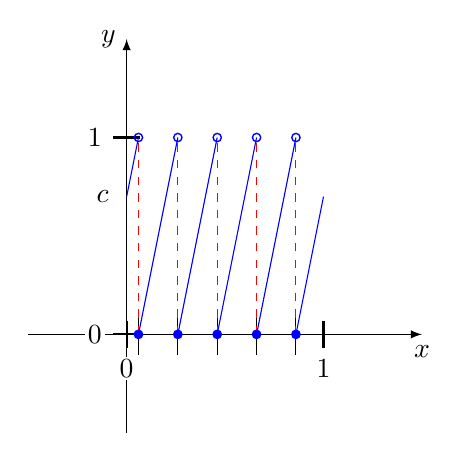
\begin{tikzpicture}[scale=2.5]
      \tkzInit[xmin = -0.5, xmax = 1, ymin = -0.5, ymax = 1]
      \tkzAxeXY
      \tkzHTick[mark=|]{0.06}
      \tkzHTick[mark=|]{0.26}
      \tkzHTick[mark=|]{0.46}
      \tkzHTick[mark=|]{0.66}
      \tkzHTick[mark=|]{0.86}
      \draw[blue] (0, 0.7) -- (0.06, 1);
      \draw[blue] (0.06, 0) -- (0.26, 1);
      \draw[blue] (0.26, 0) -- (0.46, 1);
      \draw[blue] (0.46, 0) -- (0.66, 1);
      \draw[blue] (0.66, 0) -- (0.86, 1);
      \draw[blue] (0.86, 0) -- (1, 0.7);
      \draw[red, dashed] (0.06, 0) -- (0.06, 1);
      \draw[red, dashed] (0.26, 0) -- (0.26, 1);
      \draw[red, dashed] (0.46, 0) -- (0.46, 1);
      \draw[red, dashed] (0.66, 0) -- (0.66, 1);
      \draw[red, dashed] (0.86, 0) -- (0.86, 1);
      \node [circle, draw, fill=none, line width = .5pt, color = blue, inner sep = 0pt, minimum size = 3pt] (ca) at (0.06, 1) {};
      \node [circle, draw, fill=none, line width = .5pt, color = blue, inner sep = 0pt, minimum size = 3pt] (ca) at (0.26, 1) {};
      \node [circle, draw, fill=none, line width = .5pt, color = blue, inner sep = 0pt, minimum size = 3pt] (ca) at (0.46, 1) {};
      \node [circle, draw, fill=none, line width = .5pt, color = blue, inner sep = 0pt, minimum size = 3pt] (ca) at (0.66, 1) {};
      \node [circle, draw, fill=none, line width = .5pt, color = blue, inner sep = 0pt, minimum size = 3pt] (ca) at (0.86, 1) {};
      \node [circle, draw, fill, line width = .5pt, color = blue, inner sep = 0pt, minimum size = 3pt] (ca) at (0.06, 0) {};
      \node [circle, draw, fill, line width = .5pt, color = blue, inner sep = 0pt, minimum size = 3pt] (ca) at (0.26, 0) {};
      \node [circle, draw, fill, line width = .5pt, color = blue, inner sep = 0pt, minimum size = 3pt] (ca) at (0.46, 0) {};
      \node [circle, draw, fill, line width = .5pt, color = blue, inner sep = 0pt, minimum size = 3pt] (ca) at (0.66, 0) {};
      \node [circle, draw, fill, line width = .5pt, color = blue, inner sep = 0pt, minimum size = 3pt] (ca) at (0.86, 0) {};
      \tkzText[left=3pt](0, 0.7){$c$}
    \end{tikzpicture}
  }
  \qquad
  \subfloat{
    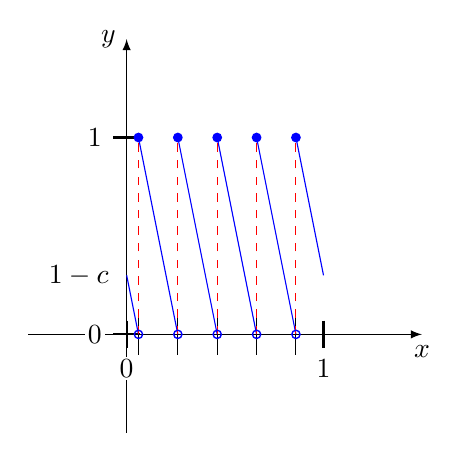
\begin{tikzpicture}[scale=2.5]
      \tkzInit[xmin = -0.5, xmax = 1, ymin = -0.5, ymax = 1]
      \tkzAxeXY
      \tkzHTick[mark=|]{0.06}
      \tkzHTick[mark=|]{0.26}
      \tkzHTick[mark=|]{0.46}
      \tkzHTick[mark=|]{0.66}
      \tkzHTick[mark=|]{0.86}
      \draw[blue] (0, 0.3) -- (0.06, 0);
      \draw[blue] (0.06, 1) -- (0.26, 0);
      \draw[blue] (0.26, 1) -- (0.46, 0);
      \draw[blue] (0.46, 1) -- (0.66, 0);
      \draw[blue] (0.66, 1) -- (0.86, 0);
      \draw[blue] (0.86, 1) -- (1, 0.3);
      \draw[red, dashed] (0.06, 0) -- (0.06, 1);
      \draw[red, dashed] (0.26, 0) -- (0.26, 1);
      \draw[red, dashed] (0.46, 0) -- (0.46, 1);
      \draw[red, dashed] (0.66, 0) -- (0.66, 1);
      \draw[red, dashed] (0.86, 0) -- (0.86, 1);
      \node [circle, draw, fill, line width = .5pt, color = blue, inner sep = 0pt, minimum size = 3pt] (ca) at (0.06, 1) {};
      \node [circle, draw, fill, line width = .5pt, color = blue, inner sep = 0pt, minimum size = 3pt] (ca) at (0.26, 1) {};
      \node [circle, draw, fill, line width = .5pt, color = blue, inner sep = 0pt, minimum size = 3pt] (ca) at (0.46, 1) {};
      \node [circle, draw, fill, line width = .5pt, color = blue, inner sep = 0pt, minimum size = 3pt] (ca) at (0.66, 1) {};
      \node [circle, draw, fill, line width = .5pt, color = blue, inner sep = 0pt, minimum size = 3pt] (ca) at (0.86, 1) {};
      \node [circle, draw, fill=none, line width = .5pt, color = blue, inner sep = 0pt, minimum size = 3pt] (ca) at (0.06, 0) {};
      \node [circle, draw, fill=none, line width = .5pt, color = blue, inner sep = 0pt, minimum size = 3pt] (ca) at (0.26, 0) {};
      \node [circle, draw, fill=none, line width = .5pt, color = blue, inner sep = 0pt, minimum size = 3pt] (ca) at (0.46, 0) {};
      \node [circle, draw, fill=none, line width = .5pt, color = blue, inner sep = 0pt, minimum size = 3pt] (ca) at (0.66, 0) {};
      \node [circle, draw, fill=none, line width = .5pt, color = blue, inner sep = 0pt, minimum size = 3pt] (ca) at (0.86, 0) {};
      \tkzText[left=3pt](0, 0.3){$1 - c$}
    \end{tikzpicture}
  }
  \caption{Graphs of $x \mapsto \{ax + c\}$ and $x \mapsto 1 - \{ax + c\}$ for $a = 5$ and $c = 0.7$.}
  \label{fig:graph2}
\end{figure}

\begin{proof}
By \Cref{lem:triangle-group}, there is some odd number \(a \in \mathbb{Z}\) such that \(f'(x)\) is \(a\) for all \(x\) except for a finite number of values. Let \(f(0) = c\), then by \Cref{lem:triangle-group} again we have \(f(x)\) equal to \(ax + c\) modulo 1 for all \(x \in S^1\). Let \(g : S^1 \to \mathbb{R}\) be the function \(g(x) = \{ax + c\}\). Then for every \(x \in S^1\), as the value \(f(x)\) is nonnegative and equal to \(ax + c\) modulo 1, we have \(f(x) \geq g(x) \geq 0\). But note that the integral \(\int g\) is exactly equal to \(1/2\) (see \Cref{fig:graph2}). So \(f\) and \(g\) should be equal almost everywhere. As \(f\) is right-continuous by \Cref{lem:triangle-group}, \(f(x)\) should be equal to the right limit \(g(x -)\) of \(g\).
If \(a > 0\), then \(g\) is right-continuous so \(f(x) = g(x) = \left\{ ax + c \right\}\). If \(a < 0\), then the right limit of \(g\) is \(1 - \left\{ -ax + \left\{ - c \right\} \right\}\) (this is the value in \((0, 1]\) equal to \(ax + c\) modulo 1).
\end{proof}

We now finish the proof of \Cref{thm:triangle-cover}. By \Cref{lem:triangle-unit-area}, the discontinuities of \(g = \sum_{i=0}^n f_{T_i} - \sum_{j=1}^n f_{S_j}\) have to be equidistributed in \(S^1\) with a gap of \(1/a\) for some positive odd number \(a\).
But each \(T_i\) can be taken arbitrary as it contains the smaller triangle \(T_i'\) of side \(< 1\). So take each \(T_i\) so that the rescaled \(y\)-coordinates \(z_{T_0}, z_{T_1}, \dots, z_{T_n}\) are different from \(z_{S_1}, z_{S_2}, \dots, z_{S_n}\) modulo 1 and \(z_{T_1} - z_{T_0}\) is an irrational number.
Then \(g\) has discontinuities at \(z_{T_0} + \mathbb{Z}, z_{T_1} + \mathbb{Z}, \dots, z_{T_n} + \mathbb{Z} \in S^1\), and two of them has an irrational gap. This gives contradiction and finishes the proof.

\section{Proof of \Cref{thm:max-epsilon}}

The group $\mathcal{T}$ was the key of the proof of the main \Cref{thm:triangle-cover}.
We use the same idea to determine the maximum $\varepsilon > 0$ such that the vertical triangle $T$ of side $n + \varepsilon$ can be covered by $n^2+2$ vertical unit equilateral triangles.

We first examine the first construction of \cite{conway2004coverup, conway2005covering} to show that it is possible to cover $T$ with $\varepsilon = 1/(n+1)$.
In the construction of \Cref{fig:triangle1}, the bottom trapezoid of left and right side $1 + \varepsilon$ and bottom side $n + \varepsilon$ is covered by $2n+1$ unit equilateral triangles.
The $n$ unit triangles at the very bottom directed upwards has bottom sides added to a line segment of length $1 + n(1 - \varepsilon)$.
For the construction to work, we need $n + \varepsilon \leq 1 + n(1 - \varepsilon)$ and 
by solving we get $\varepsilon \leq 1/(n+1)$.

Now we show that if $\varepsilon > 1/(n+1)$ then it is impossible to cover $T$ with $n^2+2$ vertical unit equilateral triangles.
Without loss of generality, assume that the bottom side of $T$ is the $x$-axis so that the rescaled coordinate $y_T$ is equal to zero.
Let $\tilde{f}_T$ be the function defined as \Cref{def:projection-ftn}.

\printbibliography


\end{document}